\documentclass[12pt]{article}

% Language setting
% Replace `english' with e.g. `spanish' to change the document language
\usepackage[english]{babel}

% Set page size and margins
% Replace `letterpaper' with `a4paper' for UK/EU standard size
\usepackage[letterpaper,top=2cm,bottom=2cm,left=3cm,right=3cm,marginparwidth=1.75cm]{geometry}

% Useful packages
\usepackage{mathptmx} %% For TImes New Roman Font
\usepackage{amsmath}
\usepackage{graphicx}
\usepackage[colorlinks=true, allcolors=blue]{hyperref}
%\usepackage{fancyhdr}

\title{Title: Clinical Diagnosis of Cardiovascular Disorder using Machine Learning to Classify Heart Sounds }
\author{Design Contest, VLSID 2025, Bengaluru}

\begin{document}
\maketitle

\begin{abstract}

\end{abstract}

%%%--- HARDWARE PLATFORM
\section{Hardware Platform}

\subsubsection*{Microchip Technology’s RISC-V based PolarFire SoC Icicle Kit}

The \href{https://www.microchip.com/en-us/development-tool/mpfs-icicle-kit-es}{PolarFire SoC Icicle Kit} is a low-cost platform for evaluating the five-core Linux-capable RISC-V microprocessor subsystem, real-time execution, low-power capabilities, and peripherals of the PolarFire SoC FPGA. PolarFire SoC is ideal for power-efficient computing in applications such as audio, AI/ML, industrial automation, and IoT. The Icicle kit includes onboard memories (LPDDR4, SPI, eMMC flash) for Linux, a multi-rail power sensor, PCIe root port, Raspberry Pi, mikroBUS expansion ports, and various wired connectivity options for prototyping.


%%%--- EXPLANATION OF IDEA
\section{Explanation of the Idea}
% Include a block diagram, overview of implementation  (Minimum font size: 10pt, Times New Roman font. Maximum two pages including tables, diagram, references (if any) )

%%% FIGURE: KWS ARCHITECTURE
%%% ------------------------
\begin{figure}[htbp]	
    %\centerline{\includegraphics{figs/KWS-architecture.png}}
    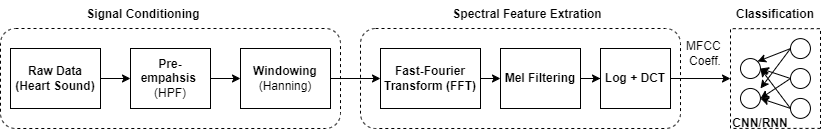
\includegraphics[width=1.0\textwidth]{figs/HSC-arch.png}
    \caption{Heart sound classification architecture.}
    \label{fig:arch-heart-sound}
\end{figure}

Identifying cardiac disorders at an early stage continues to be a vital and key approach to the diagnosis of cardiovascular disease, recognized as a primary cause of mortality \cite{members2016heart}.  
The sound signals of the heart contain information relevant to cardiovascular disorders, which has been shown to be effective in the early identification of latent heart disease \cite{yuenyong2011framework}. Historically, medical professionals have used heart sound through \textit{auscultation} to detect cardiac disorders.
Auscultation is a clinical method that is used to hear the internal sounds of the body, usually through the use of a stethoscope. It is often used to inspect the circulatory, respiratory, and gastrointestinal systems.
It is non-invasive, cost-effective, and requires minimal equipment, making it ideal for cardiac exams in small clinics or for use at home.
However, in reality, auscultation of heart sounds is heavily dependent on the experience and skills of physicians.
Cardiologists achieve an auscultation accuracy of around 80\% \cite{strunic2007detection}, while general physicians generally have an accuracy ranging from 20\% to 40\%.\cite{lam2018factors}. Computer-aided analysis through signal processing and machine learning has significantly narrowed this gap, offering enhanced tools to general physicians for more accurate diagnosis.

The standard procedure for classifying heart sounds is shown in Figure~\ref{fig:arch-heart-sound} \cite{gupta2007neural, nguyen2023heart}. It comprises three main steps: 1) signal conditioning, 2) extraction of spectral features, and 3) classification. This method is a proven method in the audio world, specifically keyword spotting (KWS) \cite{chong20220}.
 
\section{Example of its Application}
% application (Describe an example consisting of potential application/Future application. This will enable usage model towards its market acceptance) (maximum 200 words)


\section{Benefits and Value Addition}
% (Explain the key benefits of your idea/implementation. You should describe the key value addition of your idea as this will explain why your idea has value in the presence of other participants. It will show uniqueness/Unique selling point/key differentiator) (maximum 200 words)




\section{Team Members}
% •	List your team members’ names, program, department, year of study and contact emails here
\begin{table}[h]
    \centering
    \begin{tabular}{|c|c|c|c|c|}
        \hline
        \textbf{Name} & \textbf{Program} & \textbf{Dept.} & \textbf{Year} & \textbf{Email} \\ \hline\hline
        & & & & \\ \hline
        & & & & \\ \hline
        & & & & \\ \hline
        & & & & \\ \hline
    \end{tabular}
    \caption{Team Member Information}
    \label{tab:student_info}
\end{table}

\section{University Address}
% •	Include the name of your university/college and your institute’s postal address to ship the boards
Silicon University \\
Silicon Hills Road, Patia \\
Bhubaneswar, 751024, ODISHA

\section{Contact Person}
%  Mention one contact person from the institute, his/her official/institute email id, and contact phone number.

Saroj Rout \\
Additional Professor, Electronics Engineering Department \\
Silicon University, Odisha \\
\textit{Email}: \texttt{saroj.rout@silicon.ac.in} \\
\textit{Phone}: +91-90907-52283 \\


\bibliographystyle{ieeetr}
\bibliography{reference}

\end{document}